\documentclass[10pt, a4paper]{scrartcl}

\usepackage{vorschule}
\usepackage[
	typ=ab,
	fach=Informatik,
	lerngruppe={Q2},
	nummer=III.6,
	module={Symbole,Lizenzen,Papiertypen},
	seitenzahlen=keine,
	farbig,
	lizenz=cc-by-nc-sa-4,
]{schule}

\usepackage[
	kuerzel=Ngb,
	reihe={Nichtlineare Datenstrukturen},
	version={2020-12-02},
]{ngbschule}

\author{J. Neugebauer}
\title{Langlaufsimulator}
\date{\Heute}

\setzeAufgabentemplate{ngbohne}


\begin{document}
\ReiheTitel

\begin{center}
	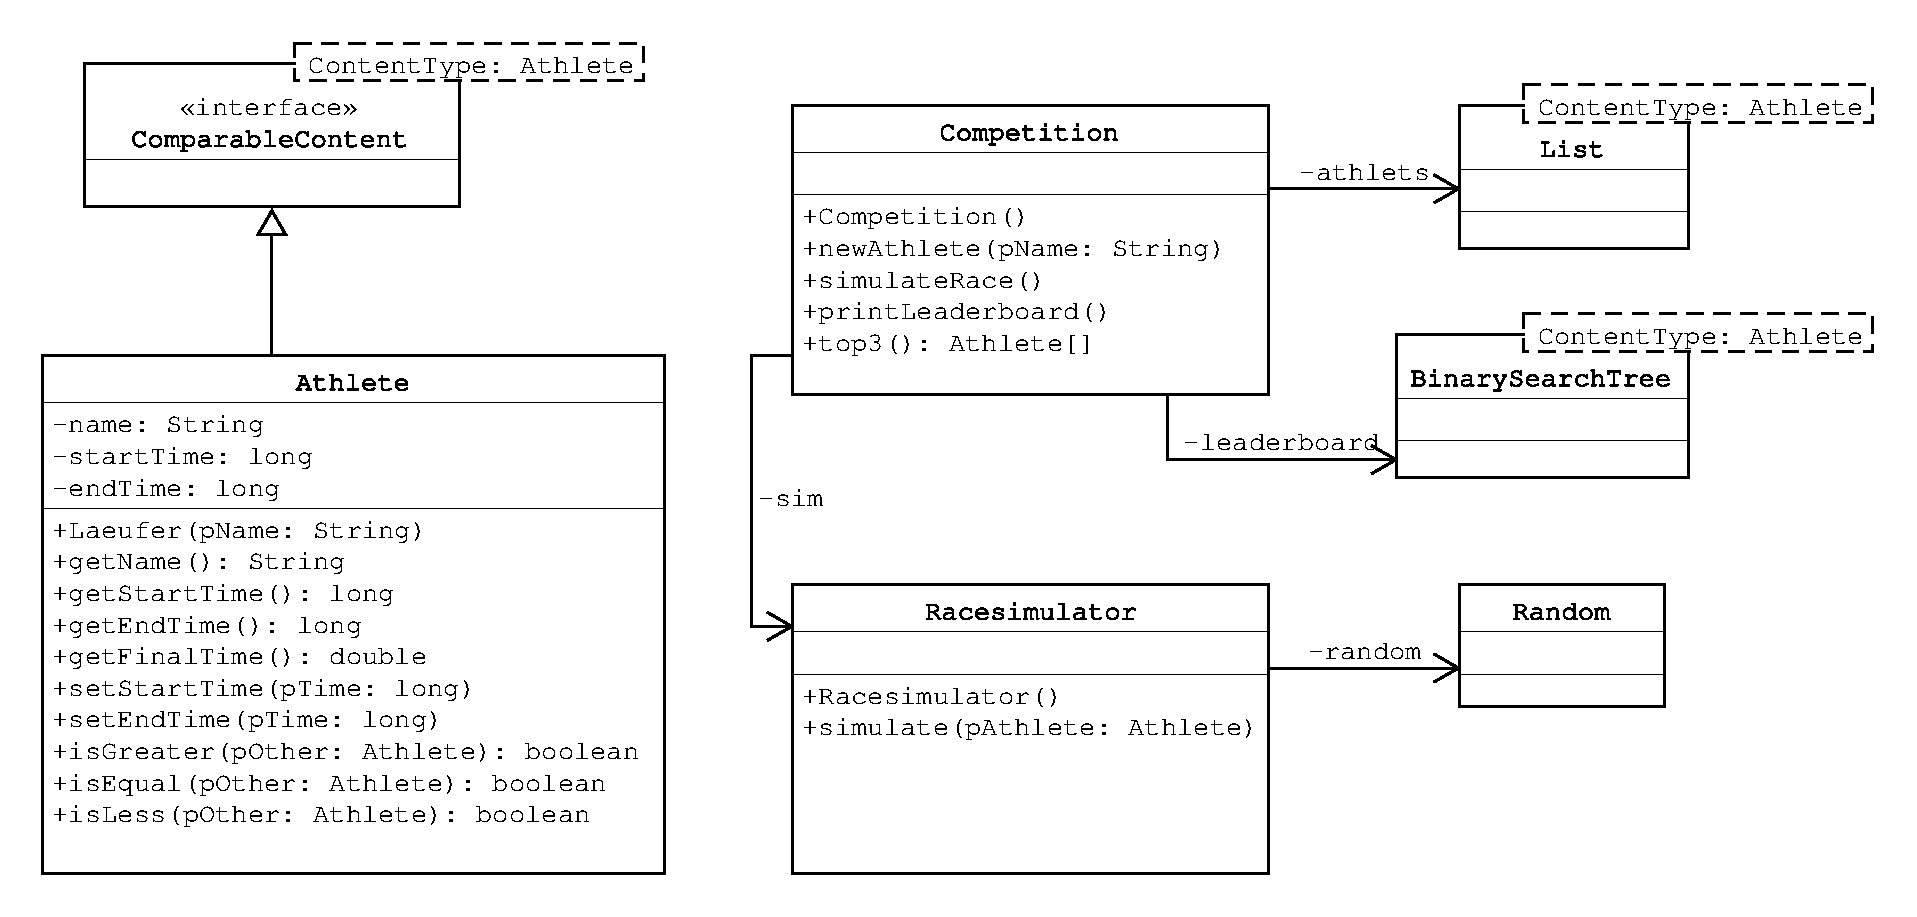
\includegraphics[width=\textwidth]{Q2-AB.III.7-Abb_UML_Langlauf}
\end{center}

\begin{aufgabe}[symbol=\symPartner\,\symLaptop]
	\begin{teilaufgaben}
		\teilaufgabe \operator{Beschreibe} die Beziehungen zwischen den einzelnen Klassen.
		\teilaufgabe \operator{Implementiere} die Langlaufsimulation anhand der Modellierung und der Klassendokumentation.
		\teilaufgabe \operator{Entscheide}, ob es sinnvoll wäre, die Rangliste (\code{leaderboard}) als lineare Liste zu modellieren, anstatt eines binären Suchbaums. Nimm dabei insbesondere Bezug zur Umsetzung der Methode\\ \code{printLeaderboard()}.
	\end{teilaufgaben}
\end{aufgabe}

\subsubsection*{Dokumentation der Klasse \code{Athlete}}
Die Klasse \code{Athlete} speichert die Renndaten eines Läufers. Sie dient hauptsächlich der Datenhaltung. 

Die Zeiten werden als Zeitstempel gespeichert. Ein Zeitstempel ist eine Zahl, die die vergangenen Millisekunden seit dem 1. Januar 1970 angibt. Mit \code{System.currentTimeMillis()} kann der aktuelle Zeitstempel abgerufen werden.

\begin{klassenDokumentation}
	\methodenDokumentation{}{public long getStartTime()}{
		Gibt den Zeitstempel der Startzeit des Läufers zurück.
	}
	\methodenDokumentation{}{public long getEndTime()}{
		Gibt den Zeitstempel der Endzeit des Läufers zurück.
	}
	\methodenDokumentation{}{public void setStartTime(long pTime)}{
		Setzt die Startzeit des Läufers auf den angegebenen Zeitstempel. 
	}
	\methodenDokumentation{}{public void setEndTime(long pTime)}{
		Setzt die Endzeit des Läufers auf den angegebenen Zeitstempel.
	}
	\methodenDokumentation{}{public double getFinalTime()}{
		Berechnet die Zeit des Läufers als Differenz aus den Zeitstempeln der Start- und Endzeit auf Sekunden gerundet.
	}
	\methodenDokumentation{}{public boolean isGreater(Athlete pOther)}{
		Gibt \code{true} zurück, wenn die Zeit des Läufers größer (also langsamer) als die des Läufers \code{pOther} ist.
	}
	\methodenDokumentation{}{public boolean isEqual(Athlete pOther)}{
		Gibt \code{true} zurück, wenn die Zeit des Läufers gleich der des Läufers \code{pOther} ist.
	}
	\methodenDokumentation{}{public boolean isLess(Athlete pOther)}{
		Gibt \code{true} zurück, wenn die Zeit des Läufers kleiner (also schneller) als die des Läufers \code{pOther} ist.
	}
\end{klassenDokumentation}

\subsubsection*{Dokumentation der Klasse \code{Competition}}
Die Klasse \code{Competition} stellt einen Langlaufwettbewerb dar. Sie ist die Hauptklasse für den Simulator.

\begin{klassenDokumentation}
	\methodenDokumentation{}{public void newAthlete(String pName)}{
		Erstellt einen neuen Läufer und speichert ihn in der Liste der Teilnehmer
	}
	\methodenDokumentation{}{public void simulateRace()}{
		Simuliert ein Langlaufrennen, indem für jeden Teilnehmer mittels des \code{Racingsimulator}s eine Zeit für das Rennen generiert wird. Steht eine Zeit fest, wird der Läufer in die Rangliste eingefügt.
	}
	\methodenDokumentation{}{public void printLeaderboard()}{
		Gibt die aktuelle Rangliste des Rennens auf der Kommandozeile aus. Sortiert vom schnellsten zum langsamsten Läufer.
	}
	\methodenDokumentation{}{public Athlete[] top3()}{
		Gibt ein Array mit den drei besten Läufern des Rennens zurück. Eenn das Rennen noch nicht vollständig simuliert wurde, wird ein leeres Array zurückgegeben.
	}
\end{klassenDokumentation}

\subsubsection*{Dokumentation der Klasse \code{Racesimulator}}
Die Klasse \code{Racesimulator} erzeugt simulierte Zeiten für Läufer. Sie benutzt dafür ein Objekt der Klasse \code{java.util.Random}.

\begin{klassenDokumentation}
	\methodenDokumentation{}{public void simulate(Athlete pAthlete)}{
		Erzeugt eine Start und eine Endzeit für den Läufer \code{pAthlete}.
	}
\end{klassenDokumentation}

\end{document}
